\documentclass{standalone}
\usepackage[dvipsnames]{xcolor}
\usepackage{tikz}
\usetikzlibrary{positioning, shapes, arrows,}

\begin{document}
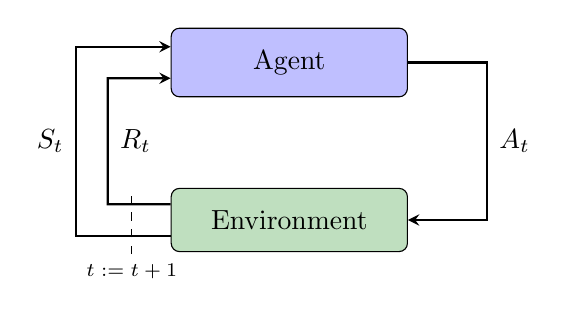
\begin{tikzpicture}[>=stealth, node distance=1cm, on grid, auto,
    entry/.style = {draw, rectangle, inner sep=8pt, rounded corners=3pt,
                    minimum width=3cm},
    arrow/.style = {thick,-stealth}]

    % States
    \node [] (center) {};
    \node [entry, fill=blue!25] (agent) [above=of center] {Agent};
    \node [entry, fill=Green!25] (env) [below=of center] {Environment};
    \node [] (time) [below left = 0.65cm and 2cm of env] {\scriptsize\(t:=t+1\)};
    \draw [dashed] (time) -- +(0,1);

    % Transitions
    \draw [arrow] (agent.east) -- +(1,0) --coordinate(A) +(1,-2) -- (env.east);
    \draw [arrow] ([yshift=-0.2cm]env.west) -- +(-1.2,0) --coordinate(S) +(-1.2,2.4) -- ([yshift=+0.2cm]agent.west);
    \draw [arrow] ([yshift=+0.2cm]env.west) -- +(-0.8,0) --coordinate(R) +(-0.8,1.6) -- ([yshift=-0.2cm]agent.west);
    \node [] () [right= 1pt of A] {\(A_t\)};
    \node [] () [left=  1pt of S] {\(S_t\)};
    \node [] () [right= 1pt of R] {\(R_t\)};
\end{tikzpicture}


\end{document}
